% Options for packages loaded elsewhere
\PassOptionsToPackage{unicode}{hyperref}
\PassOptionsToPackage{hyphens}{url}
%
\documentclass[
  12pt,
]{article}
\usepackage{lmodern}
\usepackage{amssymb,amsmath}
\usepackage{ifxetex,ifluatex}
\ifnum 0\ifxetex 1\fi\ifluatex 1\fi=0 % if pdftex
  \usepackage[T1]{fontenc}
  \usepackage[utf8]{inputenc}
  \usepackage{textcomp} % provide euro and other symbols
\else % if luatex or xetex
  \usepackage{unicode-math}
  \defaultfontfeatures{Scale=MatchLowercase}
  \defaultfontfeatures[\rmfamily]{Ligatures=TeX,Scale=1}
\fi
% Use upquote if available, for straight quotes in verbatim environments
\IfFileExists{upquote.sty}{\usepackage{upquote}}{}
\IfFileExists{microtype.sty}{% use microtype if available
  \usepackage[]{microtype}
  \UseMicrotypeSet[protrusion]{basicmath} % disable protrusion for tt fonts
}{}
\makeatletter
\@ifundefined{KOMAClassName}{% if non-KOMA class
  \IfFileExists{parskip.sty}{%
    \usepackage{parskip}
  }{% else
    \setlength{\parindent}{0pt}
    \setlength{\parskip}{6pt plus 2pt minus 1pt}}
}{% if KOMA class
  \KOMAoptions{parskip=half}}
\makeatother
\usepackage{xcolor}
\IfFileExists{xurl.sty}{\usepackage{xurl}}{} % add URL line breaks if available
\IfFileExists{bookmark.sty}{\usepackage{bookmark}}{\usepackage{hyperref}}
\hypersetup{
  pdftitle={Assignment 1 Data Science},
  pdfauthor={Sofie Brynjelsen, Silje Marie Danielsen},
  hidelinks,
  pdfcreator={LaTeX via pandoc}}
\urlstyle{same} % disable monospaced font for URLs
\usepackage[margin=1in]{geometry}
\usepackage{color}
\usepackage{fancyvrb}
\newcommand{\VerbBar}{|}
\newcommand{\VERB}{\Verb[commandchars=\\\{\}]}
\DefineVerbatimEnvironment{Highlighting}{Verbatim}{commandchars=\\\{\}}
% Add ',fontsize=\small' for more characters per line
\usepackage{framed}
\definecolor{shadecolor}{RGB}{248,248,248}
\newenvironment{Shaded}{\begin{snugshade}}{\end{snugshade}}
\newcommand{\AlertTok}[1]{\textcolor[rgb]{0.94,0.16,0.16}{#1}}
\newcommand{\AnnotationTok}[1]{\textcolor[rgb]{0.56,0.35,0.01}{\textbf{\textit{#1}}}}
\newcommand{\AttributeTok}[1]{\textcolor[rgb]{0.77,0.63,0.00}{#1}}
\newcommand{\BaseNTok}[1]{\textcolor[rgb]{0.00,0.00,0.81}{#1}}
\newcommand{\BuiltInTok}[1]{#1}
\newcommand{\CharTok}[1]{\textcolor[rgb]{0.31,0.60,0.02}{#1}}
\newcommand{\CommentTok}[1]{\textcolor[rgb]{0.56,0.35,0.01}{\textit{#1}}}
\newcommand{\CommentVarTok}[1]{\textcolor[rgb]{0.56,0.35,0.01}{\textbf{\textit{#1}}}}
\newcommand{\ConstantTok}[1]{\textcolor[rgb]{0.00,0.00,0.00}{#1}}
\newcommand{\ControlFlowTok}[1]{\textcolor[rgb]{0.13,0.29,0.53}{\textbf{#1}}}
\newcommand{\DataTypeTok}[1]{\textcolor[rgb]{0.13,0.29,0.53}{#1}}
\newcommand{\DecValTok}[1]{\textcolor[rgb]{0.00,0.00,0.81}{#1}}
\newcommand{\DocumentationTok}[1]{\textcolor[rgb]{0.56,0.35,0.01}{\textbf{\textit{#1}}}}
\newcommand{\ErrorTok}[1]{\textcolor[rgb]{0.64,0.00,0.00}{\textbf{#1}}}
\newcommand{\ExtensionTok}[1]{#1}
\newcommand{\FloatTok}[1]{\textcolor[rgb]{0.00,0.00,0.81}{#1}}
\newcommand{\FunctionTok}[1]{\textcolor[rgb]{0.00,0.00,0.00}{#1}}
\newcommand{\ImportTok}[1]{#1}
\newcommand{\InformationTok}[1]{\textcolor[rgb]{0.56,0.35,0.01}{\textbf{\textit{#1}}}}
\newcommand{\KeywordTok}[1]{\textcolor[rgb]{0.13,0.29,0.53}{\textbf{#1}}}
\newcommand{\NormalTok}[1]{#1}
\newcommand{\OperatorTok}[1]{\textcolor[rgb]{0.81,0.36,0.00}{\textbf{#1}}}
\newcommand{\OtherTok}[1]{\textcolor[rgb]{0.56,0.35,0.01}{#1}}
\newcommand{\PreprocessorTok}[1]{\textcolor[rgb]{0.56,0.35,0.01}{\textit{#1}}}
\newcommand{\RegionMarkerTok}[1]{#1}
\newcommand{\SpecialCharTok}[1]{\textcolor[rgb]{0.00,0.00,0.00}{#1}}
\newcommand{\SpecialStringTok}[1]{\textcolor[rgb]{0.31,0.60,0.02}{#1}}
\newcommand{\StringTok}[1]{\textcolor[rgb]{0.31,0.60,0.02}{#1}}
\newcommand{\VariableTok}[1]{\textcolor[rgb]{0.00,0.00,0.00}{#1}}
\newcommand{\VerbatimStringTok}[1]{\textcolor[rgb]{0.31,0.60,0.02}{#1}}
\newcommand{\WarningTok}[1]{\textcolor[rgb]{0.56,0.35,0.01}{\textbf{\textit{#1}}}}
\usepackage{graphicx,grffile}
\makeatletter
\def\maxwidth{\ifdim\Gin@nat@width>\linewidth\linewidth\else\Gin@nat@width\fi}
\def\maxheight{\ifdim\Gin@nat@height>\textheight\textheight\else\Gin@nat@height\fi}
\makeatother
% Scale images if necessary, so that they will not overflow the page
% margins by default, and it is still possible to overwrite the defaults
% using explicit options in \includegraphics[width, height, ...]{}
\setkeys{Gin}{width=\maxwidth,height=\maxheight,keepaspectratio}
% Set default figure placement to htbp
\makeatletter
\def\fps@figure{htbp}
\makeatother
\setlength{\emergencystretch}{3em} % prevent overfull lines
\providecommand{\tightlist}{%
  \setlength{\itemsep}{0pt}\setlength{\parskip}{0pt}}
\setcounter{secnumdepth}{-\maxdimen} % remove section numbering

\title{Assignment 1 Data Science}
\usepackage{etoolbox}
\makeatletter
\providecommand{\subtitle}[1]{% add subtitle to \maketitle
  \apptocmd{\@title}{\par {\large #1 \par}}{}{}
}
\makeatother
\subtitle{Reproduserbarhet}
\author{Sofie Brynjelsen, Silje Marie Danielsen}
\date{}

\begin{document}
\maketitle

\newpage

\begin{enumerate}
\def\labelenumi{\arabic{enumi})}
\tightlist
\item
  Innledning

  \begin{enumerate}
  \def\labelenumii{\arabic{enumii})}
  \setcounter{enumii}{1}
  \tightlist
  \item
    Definisjoner
  \end{enumerate}
\item
  Publication bias
\item
  Type 1 error

  \begin{enumerate}
  \def\labelenumii{\arabic{enumii})}
  \setcounter{enumii}{1}
  \tightlist
  \item
    Publication bias and meta-analysis
  \item
    The replication crisis
  \end{enumerate}
\item
  Løsning
\item
  Avslutnning
\item
  Referanser
\item
  Appendiks
\end{enumerate}

\hypertarget{innledning}{%
\section{Innledning}\label{innledning}}

I denne oppgaven skal vi ta for oss hva reproduserbarhet og
replikerbarhet er. Samt problemet med reprodusering.

I dagens samfunn er vitenskapen i utvikling, og det vil være et stort
behov for at man har tillit til forskningen som blir gjort. For å skape
tillit er det vesentlig at funnen som er blitt gjort, kan reproduseres.
Det vil si at når en gjennomfører samme analyse basert på samme data,
vil man endre opp med de eksakt samme svarene. I forbindelse med
reproduserbarhet vil det være vesentlig å nevne replikerbarhet.
Replikerbarhet handler om at man får samme konklusjon, når man
gjennomfører samme undersøkelse med nye data. Dette omtales også som
gullstandarden når det gjelder vitenskap. vi kan se på reproduserbarhet
som nødvendig, men ikke tilstrekkelig for replikerbarhet.

Forskere har funnet ut at det til tider er vanskelig med
reproduserbarhet. I denne forbindelse nevner (Peng, 2011) at
reproduserbarhet bær være et minstekrav for at en artikkel skal
produseres.

Robus og pålitelig forskning er grunnlaget for vitesnakpelig utvikling
og fremgang. Dette avhenger av at forskernes evne til å samle inn data
fra tidligere arbeid. ``robust and reliable sciene'' omhandler at
forskningen skal være reproduserbar, replikerbar og generaliserbar. Når
det kommer til defineringen av disse uttrykkene, har det oppstått
forvirring og misforståelser. I denne fobindelse vil vi velge å definere
disse på engelsk. (Bollen et al., 2015)

\hypertarget{definisjoner}{%
\subsection{Definisjoner}\label{definisjoner}}

\emph{"\textbf{Replicability} refers to: the ability of a researcher to
duplicate the results of a prior study if the same procedures are
followed but the new data are collected.}"

\emph{"\textbf{Generalizability} refers to: wheter the results of a
study apply in other contexts or populations that differ from the
originals.}"

\emph{"\textbf{Reproducibility} refers to: the ability of a researcher
to duplicate the results of a prior study using the same materials and
prcedures used by the original investigator.}"

\emph{\emph{Reproduserbarhet}} kan også deles inn i tre hovedkategorier;
\emph{methods reproducibility}, \emph{results reproducibility} og
\emph{robustness and generalizability}.

Methods reproducibility: ``Methods reproducibility refers to the
provision of enough detail about study procedures and data so the same
procedures could, in theory or in actuality, be exactly repeated''

Results reproducibility: ``Results reproducibility (previously descrived
as replicability) refers to obtaining the same results from the conduct
of an independent study whose procedure are as closely matched to the
original experiment as possible.''

Robustness and generallzability: ``We briefly introduce these terms
because they are sometimes used in lieu of the term reproducibility.
Robustness refers to the stability of experimental conclusjon to
varaitions in either baseline assumptions or experimental procedures. It
is somewhat related to the concept of generalizability (also known as
transportability), which refers to the persistence of an effect in
settings different from and outside of an experimental framework''.

\hypertarget{publication-bias}{%
\section{Publication bias}\label{publication-bias}}

Et annet problem knyttet til forskning er publiserings skeivhet også
kalt for publication bias. Dette omhandler at sannsynligheten for at en
studie skal bli publisert avhenger av konklusjonen til studiet. Etter å
ha undersøkt er det mange som har funnet ut at det er veldig få studier
som har en negativ konklusjon. Det vil si at man ikke forkaster vår null
hypotese. dette kan være et problem knyttet til at forskningen kan vise
at det ikke har noen effekt, noe som videre kan fære til at man går
glipp av viktig kunnskap. Et ``worst case scenario'' er at de
vitenskapelige skriftene blir en stor samling av type 1 error.

\hypertarget{type-1-error}{%
\section{Type 1 error}\label{type-1-error}}

Type 1 error vil si at man forkaster H0 når den i virkeligheten skal
beholdes. Et av problemene knyttet til dette tema er hvis man for
eksempel ufører like 100 studier som finner ingen effekt, og vi har en
som finner en effekt, vil det være en sjanse for at man finner en studie
i litteraturen som viser et feil resultat. Dette blir ofte omtalt som
``the File Drawer Problem'' (Rosenthal, 1979). Det vil si at de studiene
som viser at man ikke kan forkaste H0, ikke blir publiserte. Studier som
viser at man kan forkaste H0, blir publiserte. (Simmons et al., 2011)
hevder at dette er en svært kostbar feil å gjøre, da de blir liggende i
literaturen lenge. Dette vil også medføre at det blir mindre muligheter
for andre å reprodusere studiene for å se om de samsvarer. Falske
resultater vil overleve over en lang periode. et annet problem knyttet
til dette er at man kan bruke de falske positve svarene som utgangspunkt
for nye undersøkelser. Man vil da bruke store ressurser på å arbeide med
noe som ikke er riktig. Videre kan dette føre til politiske følger og
kostbare reformer som da i sin helhet er begrunnet ut ifra vitenskap som
ikke gjelder. Alt i alt vil dette svekke troverdigheten.

\hypertarget{publication-bias-and-meta-analysis}{%
\section{Publication bias and
meta-analysis}\label{publication-bias-and-meta-analysis}}

publiserings skeivhet kan videre forplante seg i metaanalyser, hvor man
tar for seg mange artikler innenfor et fagområde. hensikteten med
meta-analysis er å finne det generelle svaret ved å sammenfatte
resultatene fra den tidligere forskningen. Dersom man da bare tar med de
falske positive artiklene som blir publisert, vil dette ha stor
betydning for hvilen konklusjon man ender opp med.(Young et al., 2008)

\hypertarget{the-replication-crisis}{%
\section{The replication crisis}\label{the-replication-crisis}}

Et annet problem som angår dette tema er det som blir kalt for the
replication crisis. Dette har sine røtter innen psykologi men etter
hvert er det flere fagområder, som for eksmepel økonomi som har vist
interesse for tema. (Simmons et al., 2011) beviste at man vil føle seg
yngre ved å høre på ``When I'm sixty four'' av The beatles. Dette er
forskning som ikke stemmer, og etter dette utfallet ville de finne en
løsning på problemet når det kommer til publisering av forskning. De
innførte dermed seks ulike krav til forfatterne og fire guidelines til
redaktørene. Hovedformålet med disse kravene og guidlinesene er at man
skal kunne unngå å få slike resultat, som den tidligere nevnte
forskningen.

\hypertarget{luxf8sning}{%
\section{Løsning}\label{luxf8sning}}

Frisch (1933) var en av de første som ønsket en løsning på problemet med
replikkering og reprodusering. Han kom med et forslag om at de
statistike eller andre nummerisk arbeid, som skal presenteres i den
ledende tiddskriften Econometrica, må ha med originale rådata og at de
blir publiserte sammen med artiklene, med mindre de er omfattene og
store. Dette ble et stort problem ettersom regresjon var et stort om
omfattende arbeid og de ble vanskelige å flytte fra en maskin til en
annen. Det vil si at replikering og reproduksjon ble umulig. JMCB
gjennomførte også et prosjekt hvor de ville kjøre en replikasjon på
innsendte dataset som følgte med artikler som var blitt publiserte. De
undersøkte mer enn 70 arbeid og klarte å direkte reprodusere to av dem.
Mange av de publiserte arbeidene var umulige å gjenprodusere på grunn av
mangel på data.

Et forslag til å løse problemene med reprodusering av data, var å få
arkiver i journalene som ble brukt. Man akriverer koder for å regne ut
tester og modeller, noe som har vært brukt over lang tid. Senere fant
McCullough et al. (2008) ut at dette ikke fikset problemet vårt med
reprodusering av den grunn at det ikke finnes noe data. Senere i 2013,
fant de en annen mer teoretisk løsning på problemet. Ved å lage et stort
felles register der man registrerer dataene som er samlet inn.

En annen løsning på problemet er kalt for \emph{computable documents}.
Dette omhandler at koden er en del av artikkelen som har blitt
publisert. Den vil da ligge inne i de opprinnelige dokumentene som er
blitt tilsendt til til tidskriftene. Man vil dermed ha en kode til å
lese inn data, en kode for å regne ut og behandle dem, samt koder til å
teste dem og til å rapportere resultatene. Ideen er inspirert av Knuth
(1992) som ville forbedre kvaliteten på dataprogrammer og kvaliteten på
kodene. Ramsey (n.d.) laget et program kalt for Noweb, som skulle være
med på å gjøre det enklere løsning som skulle brukes på mange
forskjellige programmeringsspråk. Dette kan bidra til å øke kvaliteten.

Gentleman and Lang (2007) var opptatt av at det er essensielt å
intregere beregningene og kodene som ble brukt i dataanalysen, med selve
dokumentet og beskrivelsene av funnene. De innførte dermed et
kompenndium ``computable documents'' som skal være en samling av ulike
elementer, tekst, kode dataene, i tillegg til at de skal kunne pakkes i
ein enhet slik at det skal være enkelt å repdorusere resultatene. Får en
til dette med disse kompendiene er en godt på vei til repdouserbar
forskning.

\textbf{\emph{Dynamisk dokument}} i kompmendiene er en ordnet
sammensettning av chuncks stykker med kode og stykker med tekst. Og at
disse her kodestykkene ikke nødvnedigvis trenger å bli uført
sekvensielt. Disse kan ha avanserte strukturer. I 2005 gjennomførte
gentleman en case sudy for å vise at dette var gjennomførtbart.

\hypertarget{avslutning}{%
\subsection{Avslutning}\label{avslutning}}

Vi kan konkludere med at det kan være en utfordring ved at rapporter
skal være 100\% repoduserbare om en ikke har tilgang til kodene, og
samme rådata som ble brukt i tildligere studier. I tillegg kan det
oppstå problemer som publiserings skjeivhet, samt type 1 error, som er
nevnt tidligere. Er R notebook et godt verktøy som kan brukes til at det
skal bli mulig at vitenskaplig studier kan være reproduserbare og en kan
unngå slike problmer? Ved R notebook har en redskaper til å kode, få
fram rådata, en kan dermed få frem den innformasjonen en trenger for å
vite, for å gjøre en studie reproduserbar.

\begin{Shaded}
\begin{Highlighting}[]
\KeywordTok{sessionInfo}\NormalTok{()}
\end{Highlighting}
\end{Shaded}

\begin{verbatim}
## R version 4.0.2 (2020-06-22)
## Platform: x86_64-w64-mingw32/x64 (64-bit)
## Running under: Windows 10 x64 (build 18362)
## 
## Matrix products: default
## 
## locale:
## [1] LC_COLLATE=Norwegian Bokmål_Norway.1252 
## [2] LC_CTYPE=Norwegian Bokmål_Norway.1252   
## [3] LC_MONETARY=Norwegian Bokmål_Norway.1252
## [4] LC_NUMERIC=C                            
## [5] LC_TIME=Norwegian Bokmål_Norway.1252    
## 
## attached base packages:
## [1] stats     graphics  grDevices utils     datasets  methods   base     
## 
## loaded via a namespace (and not attached):
##  [1] compiler_4.0.2  magrittr_1.5    tools_4.0.2     htmltools_0.5.0
##  [5] yaml_2.2.1      stringi_1.4.6   rmarkdown_2.3   knitr_1.29     
##  [9] stringr_1.4.0   xfun_0.16       digest_0.6.25   rlang_0.4.7    
## [13] evaluate_0.14
\end{verbatim}

Når vi bruker \textbf{\emph{sessioninfo}} i en code-chunk. Får vi
informasjon om hvilke versjon av R studio vi har, hvilke pakker en har
lastet opp i Rstudio og samtidig andre viktig data. Når denne
informasjonen er tilgjengelig, vil det bli lettere på reprodusere
datane, og kommer til lik eller tilnermet lik konkusjon.

\hypertarget{referanser}{%
\subsection{Referanser}\label{referanser}}

\hypertarget{refs}{}
\leavevmode\hypertarget{ref-bollen2015}{}%
Bollen, K., Cacioppo, J. T., Krosnick, J. A., Olds, J. L., and Kaplan,
R. M. (2015). \emph{Social, Behavioral, and Economic Sciences
Perspectives on Robust and Reliable Science} (Report of the Subcommittee
on Replicability in Science Advisory Committee to the National Science
Foundation Directorate for Social, Behavioral, and Economic Sciences).
NSF.

\leavevmode\hypertarget{ref-frisch1933}{}%
Frisch, R. (1933). Editor's note. \emph{Econometrica}, \emph{1}(1),
1--4.

\leavevmode\hypertarget{ref-gentleman2007}{}%
Gentleman, R., and Lang, D. T. (2007). Statistical analyses and
reproducible research. \emph{Journal of Computational and Graphical
Statistics}, \emph{16}(1), 1--23.
\url{https://doi.org/10.1198/106186007X178663}

\leavevmode\hypertarget{ref-knuth1992}{}%
Knuth, D. E. (1992). \emph{Literate Programming}. Cambridge University
Press.

\leavevmode\hypertarget{ref-mccullough2008}{}%
McCullough, B. D., McGeary, K. A., and Harrison, T. D. (2008). Do
economics journal archives promote replicable research? \emph{Canadian
Journal of Economics/Revue Canadienne d'économique}, \emph{41}(4),
1406--1420. \url{https://doi.org/10.1111/j.1540-5982.2008.00509.x}

\leavevmode\hypertarget{ref-peng2011}{}%
Peng, R. D. (2011). Reproducible Research in Computational Science.
\emph{Science}, \emph{334}(6060), 1226--1227.
\url{https://doi.org/10.1126/science.1213847}

\leavevmode\hypertarget{ref-ramsey}{}%
Ramsey, N. (n.d.). \emph{Noweb home page}.

\leavevmode\hypertarget{ref-rosenthal1979}{}%
Rosenthal, R. (1979). \emph{The file drawer problem and tolerance for
null results.} \emph{86}, 638--641.

\leavevmode\hypertarget{ref-simmons2011}{}%
Simmons, J. P., Nelson, L. D., and Simonsohn, U. (2011). False-positive
psychology: Undisclosed flexibility in data collection and analysis
allows presenting anything as significant. \emph{Psychological Science},
\emph{22}(11), 1359--1366.
\url{https://doi.org/10.1177/0956797611417632}

\leavevmode\hypertarget{ref-young2008}{}%
Young, N. S., Ioannidis, J. P. A., and Al-Ubaydli, O. (2008). Why
Current Publication Practices May Distort Science. \emph{PLoS Medicine},
\emph{5}(10), e201. \url{https://doi.org/10.1371/journal.pmed.0050201}

\hypertarget{appendiks}{%
\subsection{Appendiks}\label{appendiks}}

\begin{figure}
\centering
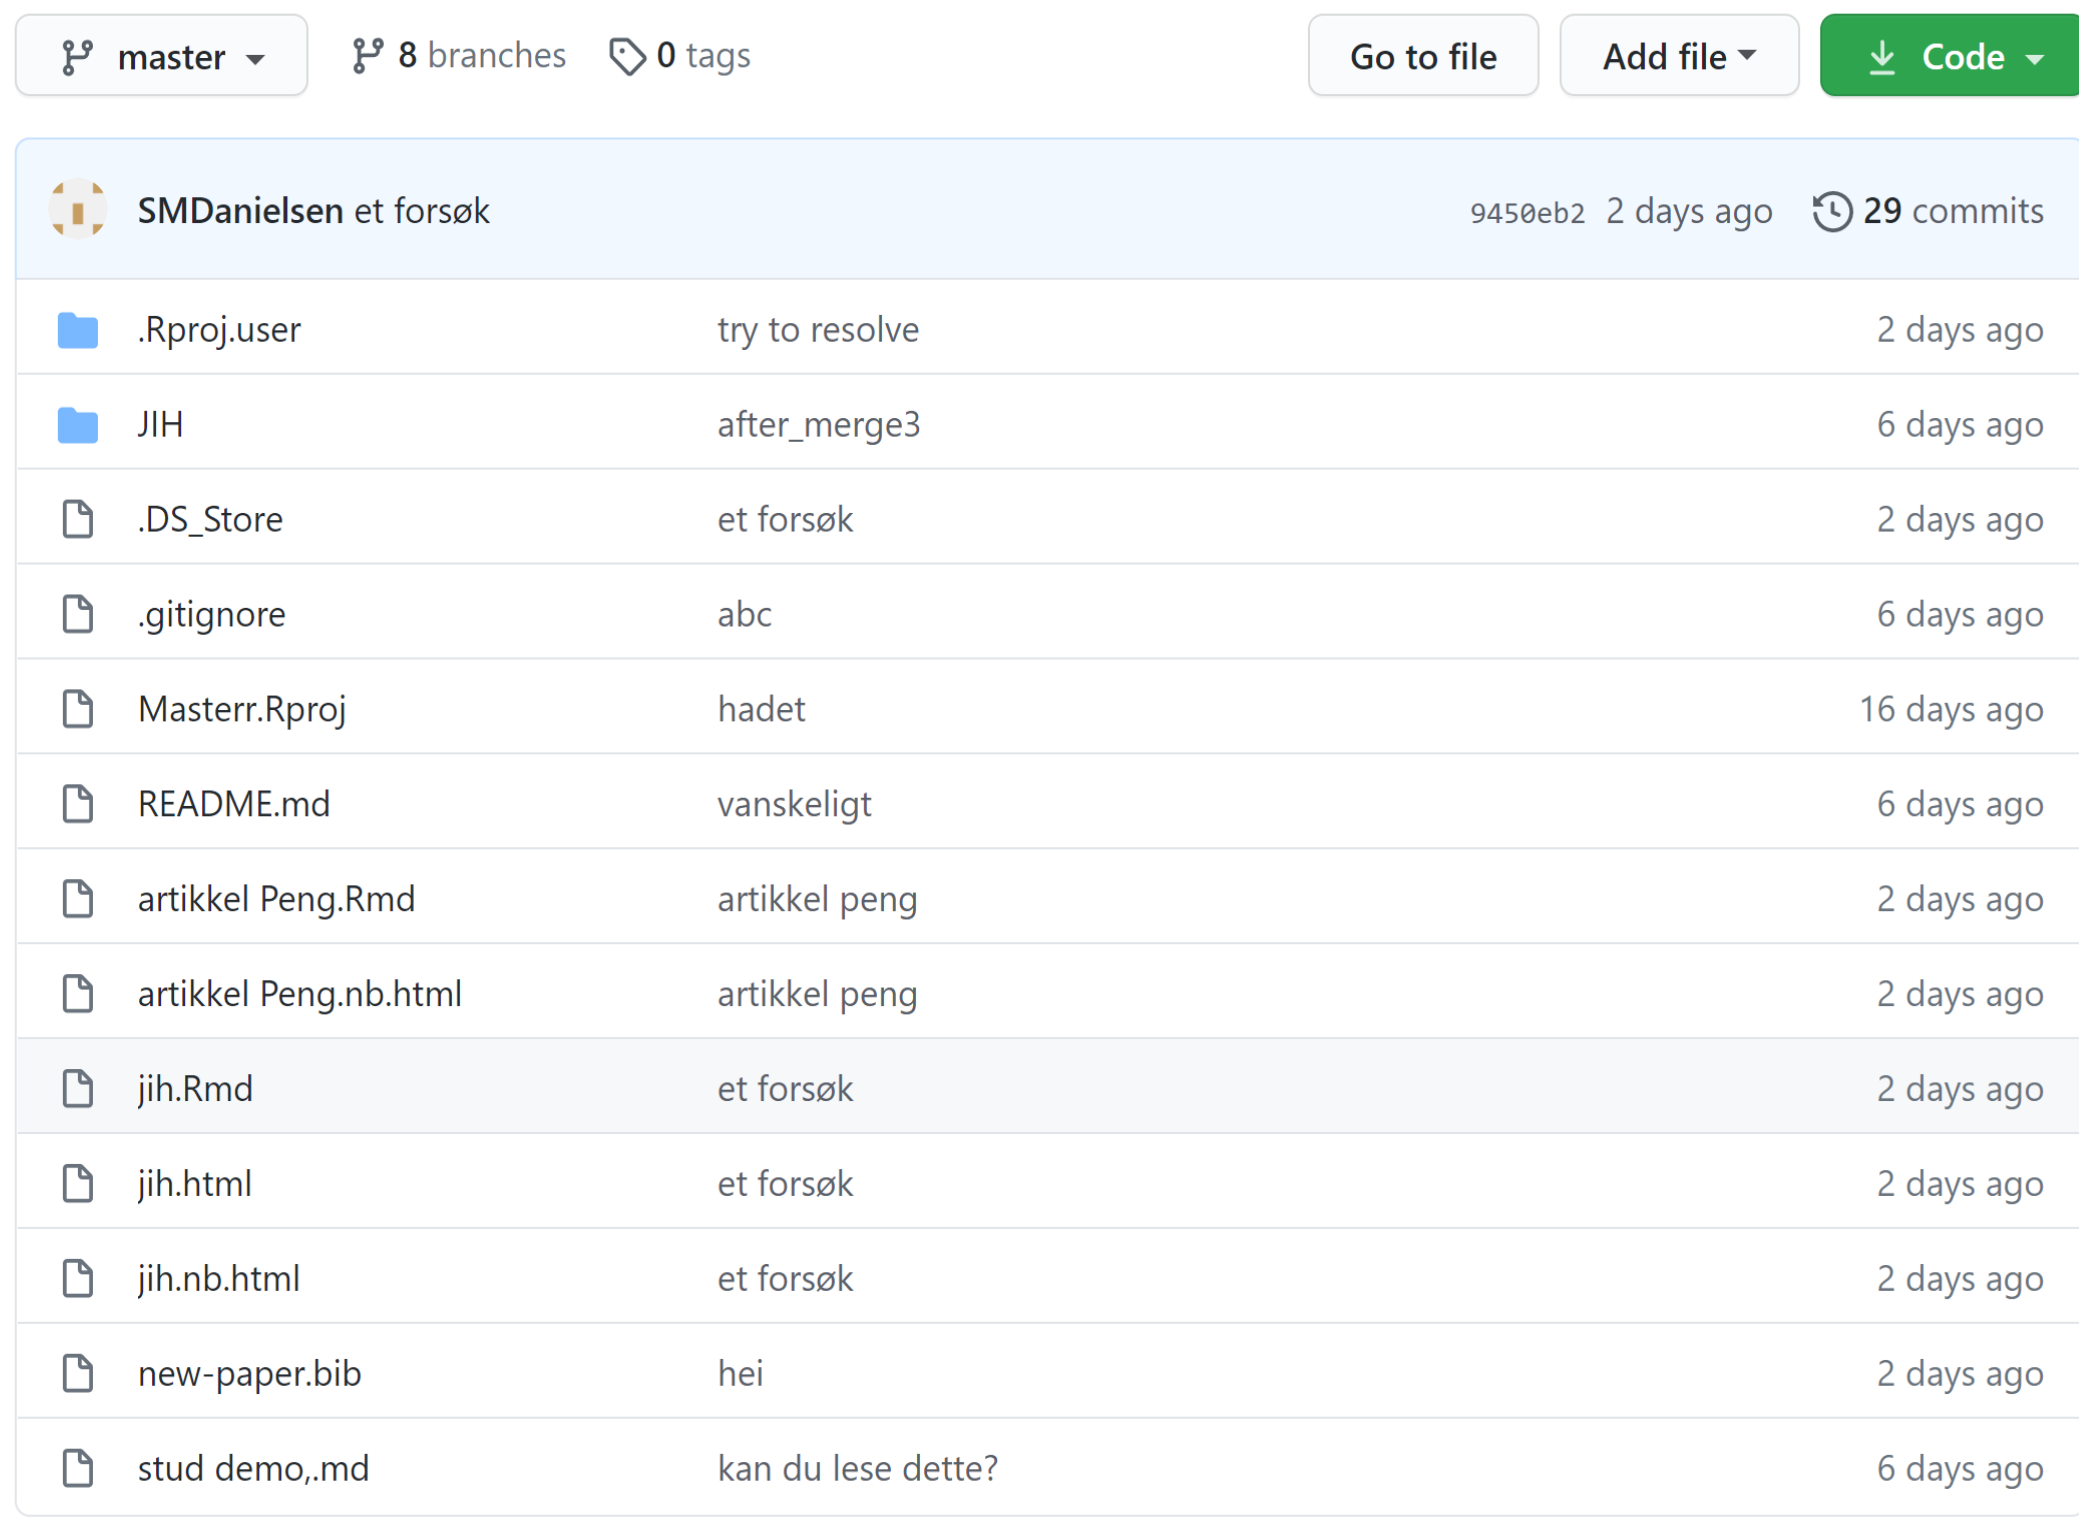
\includegraphics{commit.png}
\caption{commit history}
\end{figure}

\end{document}
